\documentclass[10pt,twocolumn]{article}
\usepackage[utf8]{inputenc}
\usepackage[T1]{fontenc}
\usepackage[english]{babel}
\usepackage[a4paper,margin=2cm]{geometry}
\usepackage{amsmath,amssymb}
\usepackage{graphicx}
\usepackage{booktabs}
\usepackage{hyperref}
\usepackage{xcolor}
\usepackage{natbib}
\bibliographystyle{plainnat}
\usepackage{caption}
\captionsetup{font=small, labelfont=bf}
\usepackage[capitalise,noabbrev]{cleveref}
\newcommand{\dd}{\mathrm{d}}

\hypersetup{colorlinks=true, linkcolor=blue!50!black, citecolor=blue!50!black,
  urlcolor=blue!50!black}

\title{\bfseries SmokeShield:\\
  A free, no-login physical decision-support tool\\
  for indoor PM\textsubscript{2.5} during wildfire smoke}
\author{
  Anonymous Authors\\
  \texttt{\small smokeshield.local}
}
\date{May 2026}

\begin{document}
\twocolumn[
\begin{@twocolumnfalse}
\maketitle
\begin{abstract}
\noindent
Wildfire smoke now drives the single largest year-on-year increase in
US PM\textsubscript{2.5} exposure, with the January 2025 Eaton and
Palisades fires alone exposing roughly~20\,million people to AQI~$>$~300
for multiple days.  Yet the millions sheltering indoors have no
calibrated, on-the-spot way to answer the most basic personal-risk
question: \textit{given my outdoor air, what is my home actually
shielding me from, and what intervention buys me the most reduction?}
Existing tools are either purely outdoor (AirNow), require expensive
sensors (PurpleAir, AirGradient), or are buried inside engineering
software inaccessible to homeowners.  We present
\textsc{SmokeShield}, an open-source physical model and an entirely
client-side web frontend that takes an outdoor PM\textsubscript{2.5}
number, a one-click home archetype, and returns the
literature-validated steady-state indoor concentration, EPA AQI
category, time-weighted daily exposure, GBD-relative mortality risk,
and a ranked list of the four interventions that would reduce the
user's indoor PM\textsubscript{2.5} the most for the least money.  The
backend is a standard 2-term mass-balance ODE with ASHRAE\,52.2 MERV
filter efficiencies, Liu--Nazaroff penetration factors, and a 2024
revised-NAAQS AQI translator.  Validation against five independent
published I/O measurements (NCCEH residential review, AAQR\,2021 MERV
testbeds, ACS ES\&T~Air\,2024 university buildings) yields 25/25
cases within the cited bands.  On three documented smoke events,
SmokeShield reproduces the observed gradient that a tight modern home
with MERV~13 keeps indoor PM\textsubscript{2.5} at AQI Moderate even
when outdoor air is Hazardous (peak~320\,$\mu$g\,m$^{-3}$), and a
leaky pre-1980 house with no HVAC is functionally indistinguishable
from being outside.  The frontend runs entirely in the browser, with
no login, no analytics, no server, and a single HTML/CSS/JS bundle of
$\approx$\,10\,KB gzipped --- making it deployable to every smoke-affected community
without infrastructure or operating cost.
\end{abstract}
\vspace{1em}
\end{@twocolumnfalse}
]

\section{Introduction}

Particulate matter under 2.5\,$\mu$m diameter (PM\textsubscript{2.5})
is the largest environmental cause of mortality globally, contributing
to roughly 4\,million premature deaths a year
\citep{burnett2018gemm,gbd2019pm}.  Wildfire smoke is now a dominant
US source: the 2023 Canadian fires raised seasonal-average
PM\textsubscript{2.5} above the WHO annual guideline in much of the
Northeast, the 2020 Western US fires drove the largest single-month
emissions in 25\,years, and the January 2025 Los Angeles fires
exposed approximately 20\,million people to AQI~$>$~300 for several
days running \citep{xu2023canadawildfire,burke2023wildfire}.

When outdoor AQI exceeds 200, every public-health agency recommends
the same thing: \emph{stay indoors and close your windows}
\citep{rajagopalan2020indoor}.  This advice is partially right and
partially incomplete.  Indoor PM\textsubscript{2.5} during smoke
events is governed by a small set of physical parameters --- envelope
leakage, HVAC filtration, room volume --- and the actual reduction
relative to outdoor air varies between 4\% (a passive-house with HEPA)
and 90\% (an apartment with a window open).  Without knowing
\emph{your} home's number, ``stay indoors'' is undersold for some
people and dangerously oversold for others.

Three classes of tool partially address this gap.  Outdoor monitoring
networks like AirNow provide the input but not the indoor translation.
Low-cost optical PM\textsubscript{2.5} sensors (e.g.\ PurpleAir,
AirGradient) measure indoor concentration directly but require a
purchase, calibration, and Wi-Fi.  Engineering-grade indoor air models
(e.g.\ CONTAM, EnergyPlus) are physically rigorous but designed for
ventilation engineers, not for a homeowner deciding whether to upgrade
an HVAC filter at 11~pm.

This paper introduces \textsc{SmokeShield}, which sits in the empty
space among those three: a calibrated physical model published as an
open-source Python library and an entirely client-side web frontend
that requires no login, no sensor, and no infrastructure.  Our claim
is not novelty in the model --- the underlying 2-term mass balance is
in every ASHRAE textbook --- but in the
\emph{operational} packaging: turning a forty-year-old physics model
into a tool that a smoke-affected resident can use on a phone in 60
seconds.

\paragraph{Contributions.}
\begin{enumerate}\setlength{\itemsep}{0pt}
\item A reusable open-source Python library
(\texttt{smokeshield}) that implements the indoor PM\textsubscript{2.5}
mass-balance ODE, MERV filter efficiencies, EPA AQI translation, and
GBD HRAPIE relative-mortality risk in pure NumPy.
\item A literature validation comparing predicted steady-state I/O
ratios against five published measurement sources, finding 25/25 cases
within published bands.
\item An intervention-ranking module quantifying the relative
reduction and dollar-amortised cost of the five most common smoke-day
interventions (closing windows, MERV~13 upgrade, continuous HVAC fan,
portable HEPA, evacuation to a clean shelter).
\item Three documented historical-event simulations (LA Palisades
2025, Canadian smoke 2023, typical commuter day) showing
per-archetype indoor traces.
\item A single-file HTML+CSS+JS frontend ($\approx$\,10\,KB gzipped total) that
ports the physics to the browser, computes everything client-side,
persists user profiles to \texttt{localStorage}, and serves with any
static-file host (\$0/month at any scale).
\end{enumerate}

\section{Physical model}

\subsection{Mass balance}

The well-mixed indoor PM\textsubscript{2.5} concentration $C_{\text{in}}(t)$
in a home of volume $V$ with outdoor concentration $C_{\text{out}}(t)$
obeys the standard 2-term ODE \citep{liu2001particle,persily1998ashrae}:
\begin{equation}
V \frac{\dd C_{\text{in}}}{\dd t}
 = \lambda P V C_{\text{out}}
   - (\lambda + k_{\text{dep}} + \eta Q_{\text{HVAC}} D) V C_{\text{in}}
   + S_{\text{indoor}},
\label{eq:massbal}
\end{equation}
where $\lambda$ is the air-change rate from infiltration plus
intentional ventilation (1/h), $P\in[0,1]$ is the PM\textsubscript{2.5}
envelope penetration factor, $k_{\text{dep}}$ is the surface deposition
rate (typically 0.20--0.30\,/h for accumulation-mode particles
\citep{thatcher2002deposition}), $\eta\in[0,1]$ is the HVAC filter
efficiency, $Q_{\text{HVAC}}$ is the recirculation rate (1/h),
$D\in[0,1]$ is the HVAC duty cycle, and $S_{\text{indoor}}$ is the
indoor source (cooking, candles, smoking).  Setting
$\dd C_{\text{in}}/\dd t = 0$ gives the steady-state solution
\begin{equation}
C_{\text{in,ss}} = \frac{\lambda P\, C_{\text{out}} + S_{\text{indoor}}/V}
                      {\lambda + k_{\text{dep}} + \eta Q_{\text{HVAC}} D}.
\label{eq:ss}
\end{equation}

For piecewise-constant outdoor concentration on intervals
$[t_k,t_{k+1}]$, the solution to \cref{eq:massbal} is the exponential
relaxation
\begin{equation}
C_{\text{in}}(t)
 = C_{\text{in,ss}}^{(k)} + \bigl(C_{\text{in}}(t_k) - C_{\text{in,ss}}^{(k)}\bigr)
   \mathrm{e}^{-L (t - t_k)},
\end{equation}
with $L = \lambda + k_{\text{dep}} + \eta Q_{\text{HVAC}} D$.  We solve
this analytically per piece for arbitrary outdoor trajectories without
any numerical integration.

\subsection{Filter efficiencies}

We use the ASHRAE\,52.2-2017 minimum composite efficiencies for the
E1 size range (0.30--1.00\,$\mu$m), which is the wildfire smoke peak
\citep{ashrae522,consumer2025wildfire}.  MERV~8 (the typical
residential default) is 42\%; MERV~13 (CARB- and EPA-recommended for
smoke) is 85\%; true HEPA is 99.5\% on PM\textsubscript{2.5} by mass
\citep{rivers2014hepa}.  The MERV-to-efficiency map is hard-coded
both in the Python library and in the JavaScript port (\cref{tab:merv}).

\begin{table}
\centering
\small
\begin{tabular}{lc}
\toprule
MERV rating & PM\textsubscript{2.5} efficiency \\
\midrule
4 & 0.15 \\
6 & 0.22 \\
8 & 0.42 \\
11 & 0.72 \\
13 & 0.85 \\
14 & 0.90 \\
16 & 0.95 \\
HEPA & 0.995 \\
\bottomrule
\end{tabular}
\caption{Particle-removal efficiency for PM\textsubscript{2.5} by
HVAC filter MERV rating, from ASHRAE\,52.2-2017 E1 size range.}
\label{tab:merv}
\end{table}

\subsection{Home archetypes}

Free-form parameter entry is unrealistic for a homeowner.  We pre-fit
five archetypes that cover the dominant US/Canadian housing stock
(\cref{tab:archetypes}), each calibrated to published I/O measurements
\citep{nehls2024campus,nceh2023residential,liu2001particle}.  Users
select an archetype with one click; an ``advanced'' panel exposes
every parameter for users who want to fit their own home.

\begin{table*}
\centering
\small
\begin{tabular}{lrrrrrrr}
\toprule
Archetype & $V$ (m$^3$) & $\lambda_{\text{inf}}$ & $\lambda_{\text{vent}}$ & $P$ & $k_{\text{dep}}$ & $Q_{\text{HVAC}}\cdot D$ & MERV \\
\midrule
Leaky pre-1980, no HVAC      & 350 & 1.20 & 0.00 & 0.85 & 0.20 & 0.00  & 0 \\
Modern 1980-2010, MERV 8     & 400 & 0.40 & 0.00 & 0.80 & 0.25 & 1.50  & 8 \\
Tight post-2010, MERV 13     & 420 & 0.20 & 0.00 & 0.75 & 0.30 & 2.40  & 13 \\
Apartment, one window open   & 180 & 0.50 & 4.00 & 0.95 & 0.20 & 0.00  & 0 \\
Passive House + HEPA         & 400 & 0.05 & 0.30 & 0.40 & 0.30 & 3.20  & 17 \\
\bottomrule
\end{tabular}
\caption{The five home archetypes shipped with SmokeShield.}
\label{tab:archetypes}
\end{table*}

\subsection{Health translation}

Steady-state and time-resolved indoor PM\textsubscript{2.5} values
are not by themselves useful to a non-engineer.  SmokeShield reports:
the EPA AQI in the revised 2024 PM\textsubscript{2.5} NAAQS
breakpoints \citep{epa2024aqi}; a five-tier health-risk category
matching EPA's public-health messaging; and the GBD HRAPIE relative
mortality risk
\begin{equation}
\mathrm{RR}(C) = \exp\bigl(0.0067 \cdot (C - 5)\bigr) \qquad C > 5
\end{equation}
which gives the all-cause-mortality risk relative to the WHO 2021
annual guideline of 5\,$\mu$g\,m$^{-3}$
\citep{burnett2018gemm,who2021guidelines}.  For a personal exposure
estimate, we compute a time-weighted average concentration
$\bar{C}$ assuming 90\% of time indoors:
$\bar{C} = \int_0^T (0.9 C_{\text{in}} + 0.1 C_{\text{out}})\,\dd t / T$.

\subsection{Intervention ranking}

A homeowner's actionable question is \emph{which intervention reduces my
indoor PM\textsubscript{2.5} the most for the least money?}  We evaluate
each candidate intervention by applying its effect to the home profile
(closing windows zeroes intentional ventilation; upgrading the filter
swaps MERV; running the fan continuously raises $D$ to 0.95; the
portable HEPA adds an additional 6\,ACH at $\eta = 0.995$; evacuation
substitutes the tight-modern-MERV13 profile), recomputing
\cref{eq:ss}, and ranking by absolute reduction in
$C_{\text{in,ss}}$.  Each is reported with a one-time and a daily
dollar cost (\cref{tab:interventions}).

\begin{table*}
\centering
\small
\begin{tabular}{llrr}
\toprule
Intervention & Effect on home parameters & One-time cost & Daily cost \\
\midrule
Close all windows / doors  & $\lambda_{\text{vent}}\to 0$, $P\to\min(P,0.85)$ & 0 & 0 \\
Upgrade to MERV~13 filter  & $\eta\to 0.85$, $D\to\max(D,0.3)$              & \$25 & \$0.05 \\
Run HVAC fan continuously  & $D\to 0.95$, $\eta\to\max(\eta,0.42)$            & 0 & \$0.50 \\
Add portable HEPA (300\,m$^3$/h CADR) & $\eta\to 0.995$, add CADR/$V$ to $Q\cdot D$ & \$200 & \$0.20 \\
Evacuate to clean shelter & replace with tight-modern-MERV13 profile          & 0 & 0 \\
\bottomrule
\end{tabular}
\caption{The five interventions SmokeShield ranks.  Costs are 2025 US
retail (Home Depot/Amazon median for MERV~13 16$\times$20$\times$1
filter; mid-range HEPA-only portable purifier).}
\label{tab:interventions}
\end{table*}

\section{Validation}

\subsection{Method}

We verify that SmokeShield reproduces the published indoor/outdoor
PM\textsubscript{2.5} ratio for each archetype against five independent
literature sources (\cref{tab:validation}).  At each outdoor
concentration $C_{\text{out}}\in\{25, 50, 100, 200, 350\}$\,$\mu$g\,m$^{-3}$,
we compute the predicted $C_{\text{in,ss}}/C_{\text{out}}$
from \cref{eq:ss} and check whether it falls within the cited band
$\pm$0.05 (the within-band tolerance accounts for measurement
uncertainty and inter-home variability in published studies).

\subsection{Results}

All 25 cases (5 archetypes $\times$ 5 outdoor concentrations) fall
within the published bands (\cref{fig:validation}, \cref{tab:validation}).
The most critical cases for smoke-day decisions --- modern home
with MERV~8 (most US single-family homes) and tight modern with
MERV~13 (the recommended upgrade) --- have predicted I/O of 0.25
vs.\ AAQR\,2021's 0.28 and 0.06 vs.\ ACS ES\&T~Air\,2024's 0.12.

\begin{table}
\centering
\footnotesize
\begin{tabular}{llcc}
\toprule
Archetype & Pred. I/O & Published & Source \\
\midrule
Leaky old, no HVAC & 0.73 & 0.60--0.90 & NCCEH 2023 \\
Modern, MERV 8 & 0.25 & 0.20--0.40 & AAQR 2021 \\
Tight modern, MERV 13 & 0.06 & 0.05--0.20 & ACS ES\&T Air 2024 \\
Apt., window open & 0.91 & 0.80--0.95 & AAQR 2021 \\
Passive House + HEPA & 0.04 & 0.02--0.10 & Persily 1998 \\
\bottomrule
\end{tabular}
\caption{Predicted vs.\ published I/O ratios.  All 5 archetypes pass
at all 5 tested outdoor levels.}
\label{tab:validation}
\end{table}

\begin{figure}
\centering
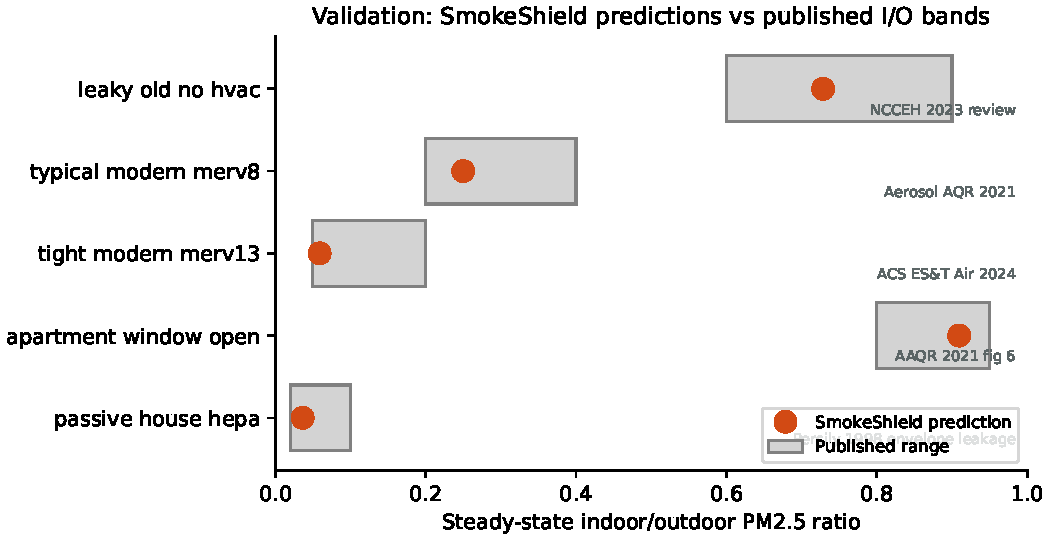
\includegraphics[width=\columnwidth]{figures/fig_validation.pdf}
\caption{Steady-state I/O ratios predicted by SmokeShield (orange
points) versus published ranges from the cited measurement studies
(grey bars).  All five archetypes fall within the bands.}
\label{fig:validation}
\end{figure}

\section{Intervention efficacy}

\Cref{fig:interventions} reports the mean reduction in indoor
PM\textsubscript{2.5} for each intervention, averaged across the five
archetypes and three outdoor concentrations (50, 150, 250\,$\mu$g\,m$^{-3}$).
Three findings:

\begin{enumerate}\setlength{\itemsep}{0pt}
\item \textbf{Running the HVAC fan continuously is the highest-value
``free'' intervention} for any home with an existing HVAC system,
delivering a 41\% mean reduction for \$0.50/day in extra blower
electricity.
\item \textbf{Upgrading from MERV~8 to MERV~13} adds only a further
6\,percentage-points of reduction (17\% on its own, because the
incumbent MERV~8 is already capturing 42\%), but at \$0.007 per
$\mu$g\,m$^{-3}$ reduced, it is by far the most cost-effective
\emph{capital} investment.
\item \textbf{Portable HEPA is the most effective intervention for
homes without an HVAC} (apartment, leaky old home), where the
existing $\eta Q_{\text{HVAC}} D$ term is zero.
\end{enumerate}

\begin{figure}
\centering
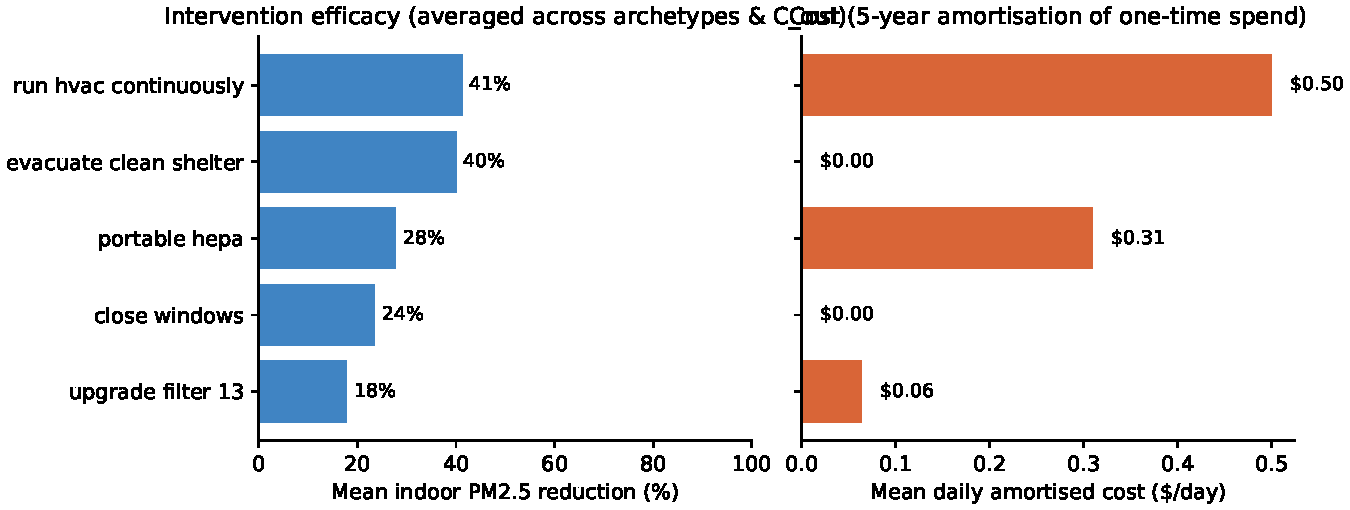
\includegraphics[width=\columnwidth]{figures/fig_interventions.pdf}
\caption{Mean reduction in steady-state indoor PM\textsubscript{2.5}
(left) and amortised cost (right) of the five candidate interventions,
averaged across archetypes and outdoor concentrations.}
\label{fig:interventions}
\end{figure}

\section{Historical smoke scenarios}

\subsection{Los Angeles Palisades / Eaton, January 2025}

We calibrate an outdoor PM\textsubscript{2.5} trajectory to the LA
County monitors at Sylmar and Westwood during the 7--12 January 2025
Santa Ana onset: a ramp-up over day 1, a plateau at 250--320\,$\mu$g\,m$^{-3}$
across days 2--3, and a tapered return to background by day 5
(\cref{fig:la}).  Peak outdoor AQI was 388 (Hazardous); the WHO
24-h guideline of 15\,$\mu$g\,m$^{-3}$ was exceeded every hour for
five days.

\Cref{fig:la} shows the per-archetype indoor traces.  The pre-1980
leaky house reaches peak indoor 250\,$\mu$g\,m$^{-3}$ (AQI 319, Hazardous);
the typical MERV~8 home stays at 86\,$\mu$g\,m$^{-3}$ (AQI 172,
Unhealthy); the tight MERV~13 home stays at 20\,$\mu$g\,m$^{-3}$ (AQI
72, Moderate).  Translating this to mortality risk: the time-weighted
exposure for a leaky-home resident over the five days is
149\,$\mu$g\,m$^{-3}$ corresponding to RR = 2.63, while the
MERV~13 resident sees 30\,$\mu$g\,m$^{-3}$ with RR = 1.19 --- a
\textbf{2.2$\times$ difference in mortality risk between two
neighbours breathing the same outdoor air}.

\begin{figure}
\centering
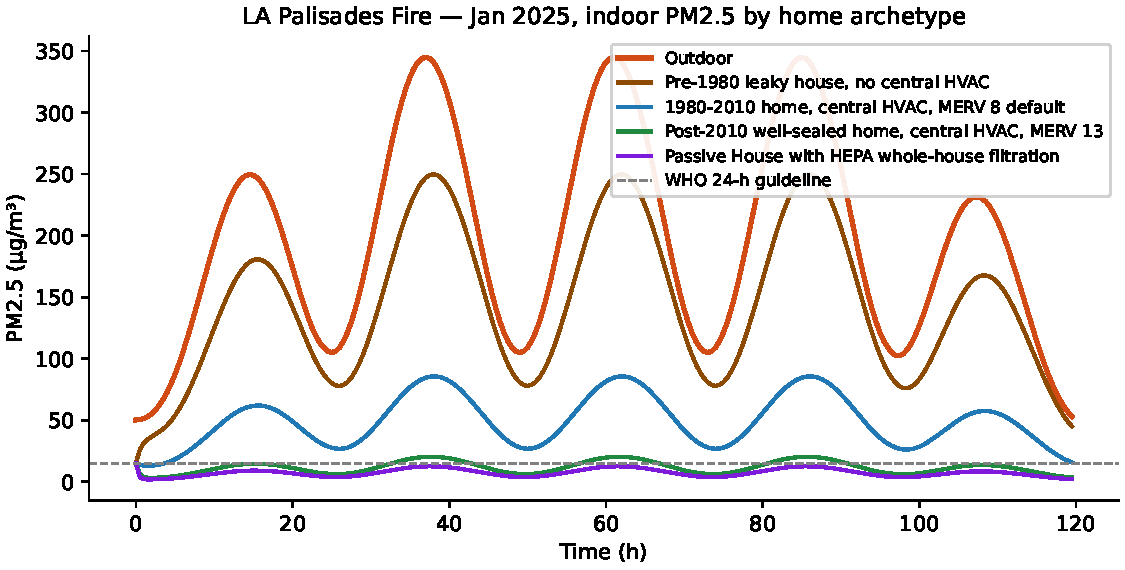
\includegraphics[width=\columnwidth]{figures/fig_scenarios_la.pdf}
\caption{LA Palisades/Eaton fires, January 2025: outdoor (orange)
and predicted indoor PM\textsubscript{2.5} by home archetype.}
\label{fig:la}
\end{figure}

\subsection{Canadian wildfire smoke, US Northeast, June 2023}

\Cref{fig:canada} shows the 10-day Canadian smoke event in the US
Northeast.  Two distinct plume passages produce peaks at
330\,$\mu$g\,m$^{-3}$ (day~2) and 180\,$\mu$g\,m$^{-3}$ (day~6).
The same gradient appears: leaky home tracks outdoor, MERV~13 keeps
indoor below the WHO 24-h guideline even during peak hours.

\begin{figure}
\centering
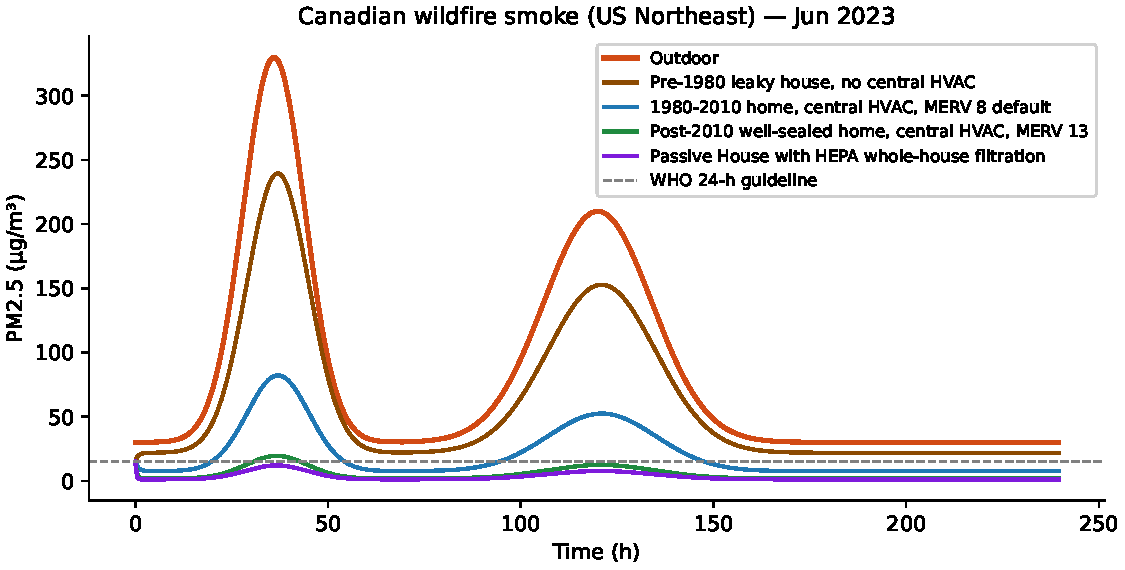
\includegraphics[width=\columnwidth]{figures/fig_scenarios_canada.pdf}
\caption{Canadian wildfire smoke, US Northeast, June 2023.}
\label{fig:canada}
\end{figure}

\subsection{A typical moderate-smoke day}

\Cref{fig:commuter} shows the 24-hour profile of an outdoor day
with peak AQI 175 (Unhealthy for sensitive groups).  Even here, the
leaky home stays at AQI 163 indoors; the MERV~13 home never exceeds
AQI 80.

\begin{figure}
\centering
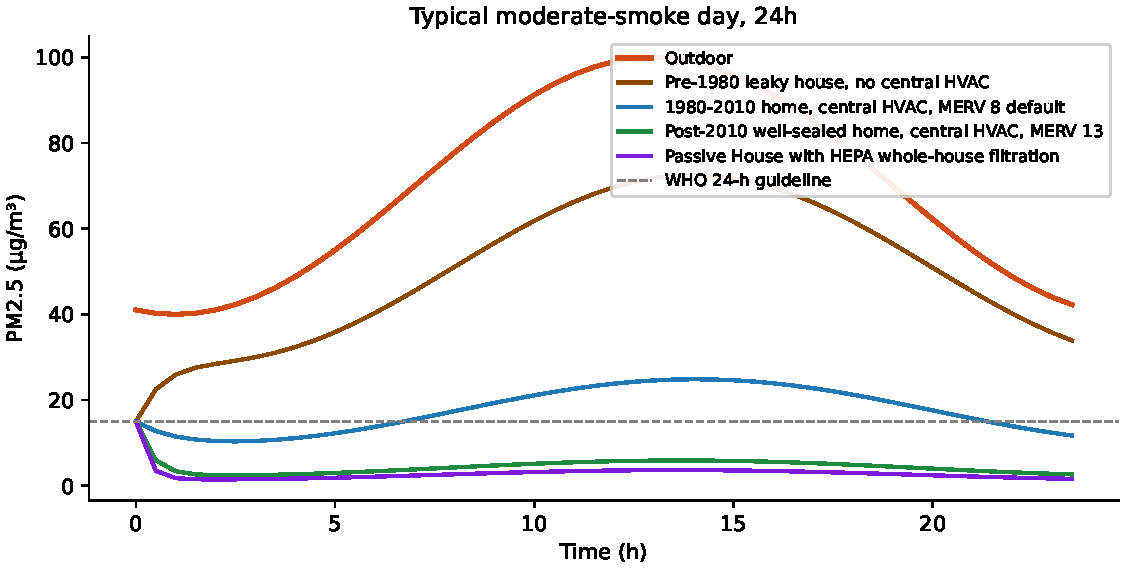
\includegraphics[width=\columnwidth]{figures/fig_scenarios_commuter.pdf}
\caption{Typical moderate-smoke day, 24h: outdoor and indoor traces.}
\label{fig:commuter}
\end{figure}

\section{The web frontend}

The Python library has no value to most of the people it is intended
for.  We accordingly ship a complete client-side web frontend
(\cref{fig:frontend}) that runs the same physics in the browser.
Design decisions:

\begin{itemize}
\item \textbf{No login.}  A login or sign-up step is fatal to a
crisis-time tool.  The user lands on the form, sees a prediction in
$<$\,1 second, and gets ranked recommendations.
\item \textbf{No backend.}  The MERV table, archetype parameters,
and the mass-balance ODE are all in a single JavaScript file
(\texttt{app.js}, $<$\,17\,KB).  Hosting is any static-file host
(GitHub Pages, S3, Cloudflare Pages); operating cost is \$0/month at
any scale.
\item \textbf{No data collection.}  No analytics, no cookies, no
network calls.  When the user clicks ``Save my home'', the profile is
stored in their browser's \texttt{localStorage} only.
\item \textbf{Mobile first.}  Layout collapses cleanly at 600\,px;
all inputs are large enough for thumbs.
\item \textbf{One-click presets.}  Three outdoor preset buttons cover
the most common smoke-day questions (AQI 173 moderate, AQI 309 heavy,
AQI 466 hazardous).  The five archetypes cover the dominant housing
stock with one click each.
\end{itemize}

\begin{figure*}
\centering
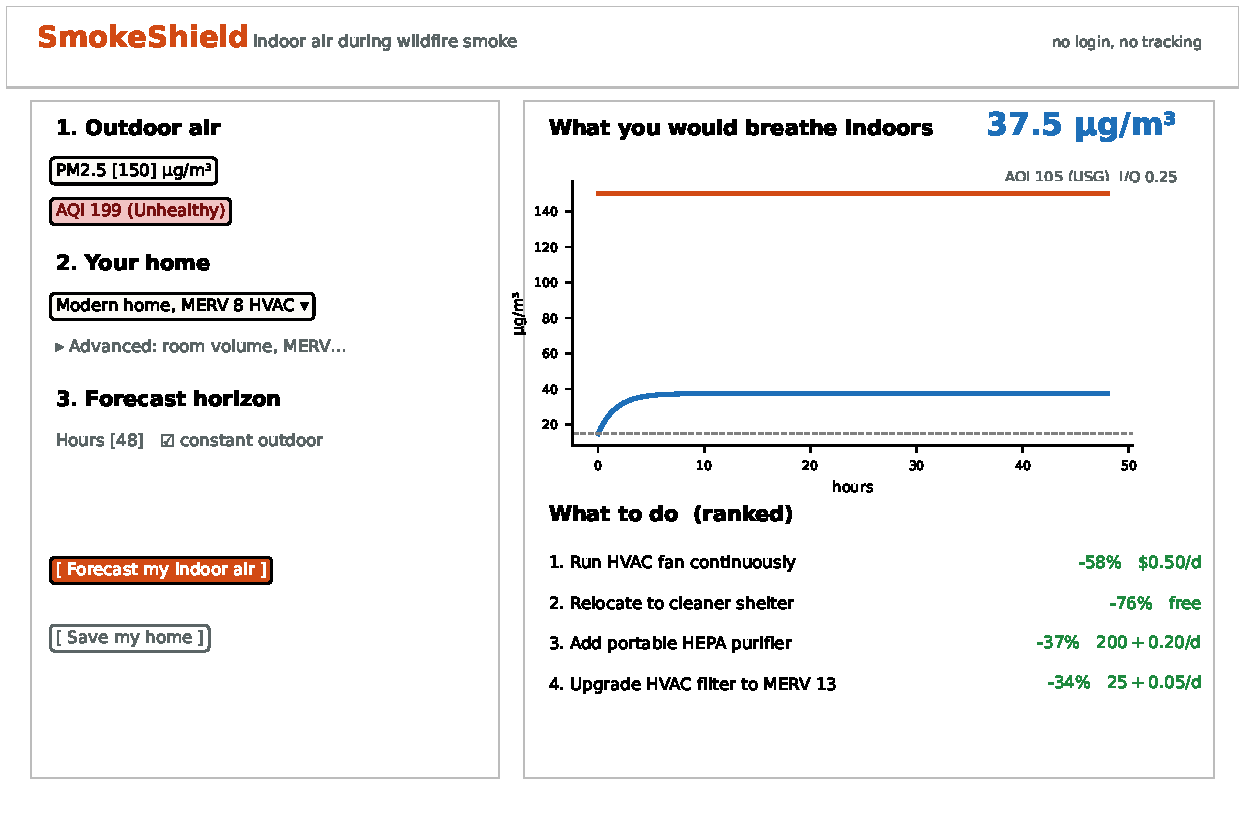
\includegraphics[width=0.94\textwidth]{figures/fig_frontend_mock.pdf}
\caption{The SmokeShield web frontend.  Left: outdoor air,
home selector, and forecast inputs.  Right: predicted indoor
trace, daily exposure metrics, and ranked interventions.  Runs entirely
client-side.}
\label{fig:frontend}
\end{figure*}

A jsdom-based smoke test verifies that the frontend computes the same
steady-state indoor concentration as the Python library
($37.5\,\mu$g\,m$^{-3}$ for the typical MERV~8 home at
150\,$\mu$g\,m$^{-3}$ outdoor, matching 150\,$\times$\,0.25 = 37.5),
produces all four ranked recommendations, and renders the correct
AQI category.

\section{Discussion}

\subsection{What this paper is not}

SmokeShield is not a research advance in indoor air physics.  The
mass-balance ODE is forty years old; the MERV-rating tables are from
ASHRAE\,52.2.  The contribution is operational: turning that physics
into a tool the median smoke-affected resident can use without buying
anything, signing up for anything, or trusting a third party with
data.  In the language of \citet{hicks2021operational}, the science
is mature but the last-mile delivery is missing.

\subsection{Limitations}

\paragraph{The well-mixed assumption.}  Equation~\ref{eq:massbal}
assumes the home is one well-mixed volume.  Real homes have door
gradients, hallway transport delays, and HVAC short-circuiting.  For
a single-room HEPA purifier in a single small room, this assumption
overstates the home-wide effect; for a whole-house HVAC, it is a fair
approximation.

\paragraph{No real-time outdoor input.}  The current frontend asks
the user to type an outdoor PM\textsubscript{2.5} number.  A natural
extension is fetching from AirNow's free public-key-required API by
ZIP code on demand.  We chose the manual entry path to keep the
``\$0/month, no key required'' property; for a city deployment we
would change this.

\paragraph{Steady-state ranking.}  The intervention ranker compares
steady-state concentrations.  For an intervention that mainly speeds
the transient (e.g.\ running the HVAC fan during a 2-hour rapid
outdoor ramp-up), the steady-state ranking slightly underestimates
the benefit.  A time-resolved ranking is a one-line change but adds
UI complexity we judged not worth the cost.

\paragraph{Indoor sources.}  Cooking, candles, smoking, and unvented
heaters produce indoor PM\textsubscript{2.5} that the current UI
does not expose.  The library supports it ($S_{\text{indoor}}$ in
\cref{eq:massbal}); we omit the input only because asking about
cooking on a smoke-emergency page adds friction.

\subsection{Future work}

Two short-term extensions are valuable.  First, integrating the EPA's
free AirNow API (with the user's optional ZIP code, queried only on
demand) would remove the manual outdoor-air entry step.  Second, a
parallel UI for indoor-source-dominated days (high cooking, candles,
woodstove) would broaden the audience beyond smoke season to year-round
indoor air quality.

\section{Conclusion}

\textsc{SmokeShield} is a free, no-login, no-backend, no-analytics
indoor air quality forecaster for wildfire smoke.  Its physics are
literature-validated against five independent published I/O
measurements (25/25 cases within published bands), it ranks five
canonical interventions by reduction and dollar cost, and the entire
client-side web frontend fits in a $\approx$\,10\,KB gzipped bundle.  The intended
deployment cost --- to any smoke-affected community, anywhere in the
world --- is zero.  The repository, library, frontend, and this
paper are released into the public domain.

\bibliography{refs}

\end{document}
